\documentclass[12pt, a4paper,  article, brazil]{abntex2}
\usepackage[utf8]{inputenc}
\usepackage[T1]{fontenc}
\usepackage{amsmath}
\usepackage{amsfonts}
\usepackage{amssymb}
%\usepackage{hyperref}  			% controla a formação do índice
%\usepackage{parskip}			% espaçamento entre os parágrafos
%\usepackage{morefloats}			% permite mais floats
\usepackage[brazil]{babel}
\addto\captionsbrazil{
	%% ajusta nomes padroes do babel
	\renewcommand{\bibname}{Refer\^encias}
	\renewcommand{\indexname}{\'Indice}
	\renewcommand{\listfigurename}{Lista de ilustra\c{c}\~{o}es}
	\renewcommand{\listtablename}{Lista de tabelas}
	%% ajusta nomes usados com a macro \autoref
	\renewcommand{\pageautorefname}{p\'agina}
	\renewcommand{\sectionautorefname}{se{\c c}\~ao}
	\renewcommand{\subsectionautorefname}{subse{\c c}\~ao}
	\renewcommand{\paragraphautorefname}{par\'agrafo}
	\renewcommand{\subsubsectionautorefname}{subse{\c c}\~ao}
	\renewcommand{\paragraphautorefname}{subse{\c c}\~ao}
}
\usepackage[alf]{abntex2cite}
\usepackage{graphicx}
%\usepackage[bottom=2cm,top=3cm,left=3cm,right=2cm]{geometry}
\title{Manual Software MadeOeste}
\author{
	Otávio A. de Almeida\\
	Cauê R. Sampaio
}
\date{\today, v 1.0}

% Espaçamentos entre linhas e parágrafos 
% O tamanho do parágrafo é dado por:
\setlength{\parindent}{1.3cm}

% Controle do espaçamento entre um parágrafo e outro:
\setlength{\parskip}{0.2cm}  % tente também \onelineskip
% compila o indice
\makeindex
\begin{document}
	\begin{center}
	\maketitle
	\begin{abstract}
		Manual para utilização do Software MadeOeste de controle de estoque.
	\end{abstract}
	\vfill
	{SOROCABA\\
	\today}
	\end{center}
	\newpage
	\tableofcontents
	\newpage
	\section{Menu Principal}
		\begin{figure}[!htb]
			\centering
			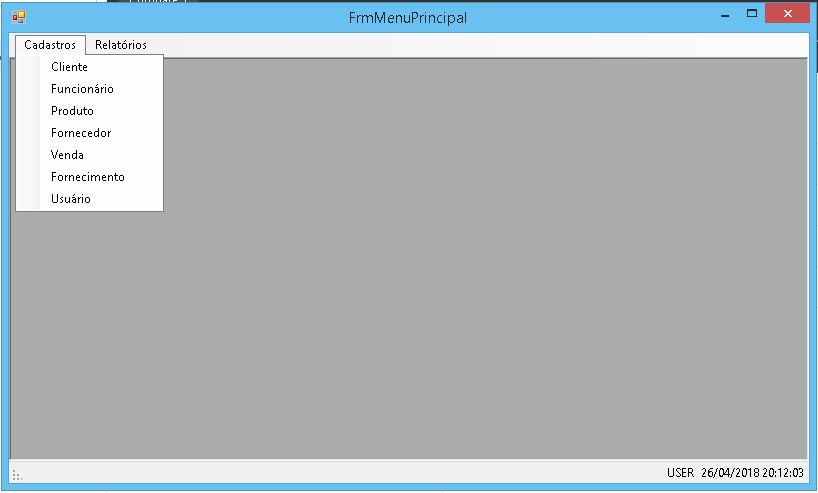
\includegraphics[scale=0.7]{../Figuras/FrmMenu.png}
			\caption{Formulário do Menu Principal}
		\end{figure}
		\subsection{Objetivo}
		O Menu do Software é o ponto de acesso para todos os demais formulários e relatórios.
		\subsection{Funcionalidades}
		\subsection{Componentes}
		Na parte superior, há da esquerda para a direita, duas abas, a aba de cadastros e a aba de relatórios.
		Na parte inferior da tela, há um menu de status que apresenta a data e hora atuais do sistema e o usuário que está logado no sistema.
		\subsubsection{Aba de Cadastros}
		Quando a aba de cadastros é pressionada, todos os índices dos formulários referentes ao sistema são exibidos, clicando em um desses índices, o formulário correspondente é aberto, caso já esteja aberto, o formulário aberto é exposto à frente dos demais.
		\subsubsection{Aba de Relatórios}
		Quando a aba de relatórios é pressionada, todos os índices dos relatórios referentes ao sistema são exibidos, clicando em um desses índices, o relatório correspondente é aberto, caso já esteja aberto, o formulário aberto é fechado e um novo é aberto para o caso de atualização de informações.
	\newpage
	\section{Formulário de Clientes}
		\subsection{Objetivo}
		O formulário de clientes tem o objetivo de cadastrar novos clientes no sistema, alterar e excluir os existentes e pesquisar os clientes cadastrados de acordo com a sua identidade.
		\subsection{Funcionalidades}	
		\subsection{Componentes}
			\subsubsection{Região de dados}
			O formulário de clientes terá uma região de dados, que ocupa a região superior esquerda da tela, destinada a inserção dados de um cliente caso a operação seja de cadastro ou alteração, ou de exibição de dados específicos caso um registro seja selecionado na tabela.
			Os componentes dessa região são:
				\begin{itemize}\itemsep1.5pt
					\item Nome do cliente
					\item A identidade do cliente, podendo ser tanto o CPF quanto o CNPJ.
					\item O e-mail do cliente
					\item O telefone principal do cliente
					\item O telefone celular do cliente
					\item O CEP do cliente
					\item A rua do cliente
					\item O número da localidade do cliente
					\item O bairro do cliente
					\item A cidade do cliente
					\item A unidade federativa do cliente
					\item As observações sobre o cliente
				\end{itemize}	
			\subsubsection{Região de operações e miscelânea}
			A região superior direita é destinada aos botões de operação, o campo de filtro por identidade e a data da informação que está selecionada na tabela.
			\subsubsection{Região da Tabela}
			A parte inferior é uma tabela que mostra todos os clientes registrados no sistema caso não haja filtro, senão ela mostra todos os clientes registrados que coincidem com o filtro.
		\newpage
\end{document}